%\documentclass[10pt,a4paper]{article}
\documentclass[12pt,a4paper]{article}
\usepackage{graphicx,amsmath}
%\usepackage{subfigure}
\usepackage{float}
\usepackage[german]{babel}
\usepackage[utf8]{inputenc}
\setcounter{secnumdepth}{4}
\usepackage[top=2cm, bottom=2.5cm, left=3cm, right=3cm]{geometry}
\begin{document}


%\title{Bachelorarbeit}
%\author{Richard Kullmann}
%\date{02.06.2017}

\thispagestyle{empty}
%\setcounter{page}{2}
\newpage
\tableofcontents
\thispagestyle{empty}
\newpage
\pagenumbering{arabic}

\section{Verhalten der Feuerrate im burstenden Zustand}
Es liegt die Vermutung nahe, dass eine Nervenzelle, die einem hohen Bias-Strom unterliegt, schneller feuert als eine Nervenzelle mit geringem Bias-Strom. Dies wird im Folgenden untersucht. F"ur den Bereich von 0 bis 4 $\mu A/cm^2$ findet sich:
\begin{figure}[H]
	\centering
	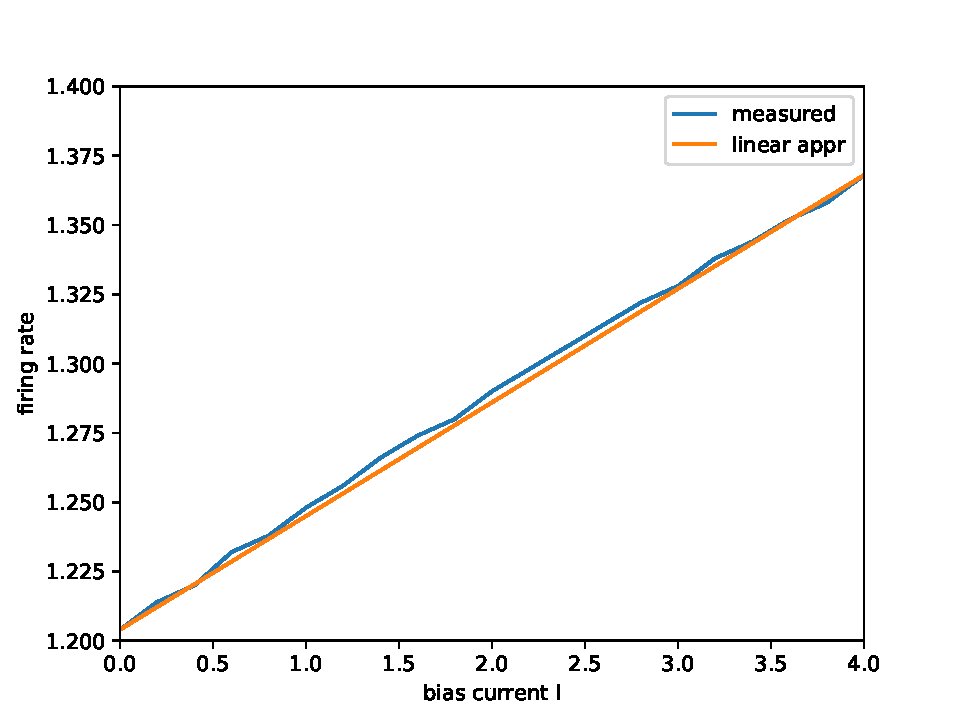
\includegraphics[scale=0.9]{detmocount04.pdf} 
	\caption{Verhalten der Feuerrate in Abh"angigkeit vom Bias}
	\label{count04}
\end{figure}
Die Feuerrate weist in dem f"ur uns interessanten Bereich st"uckweise lineares Verhalten auf. Aus diesem Grund wird diese im Folgenden linear angen"ahert.
\newpage
Wenn man jedoch einen gr"o"seren Bereich untersucht, ist zu sehen, dass der Anstieg der Kurve monoton f"allt:
\begin{figure}[H]
	\centering
	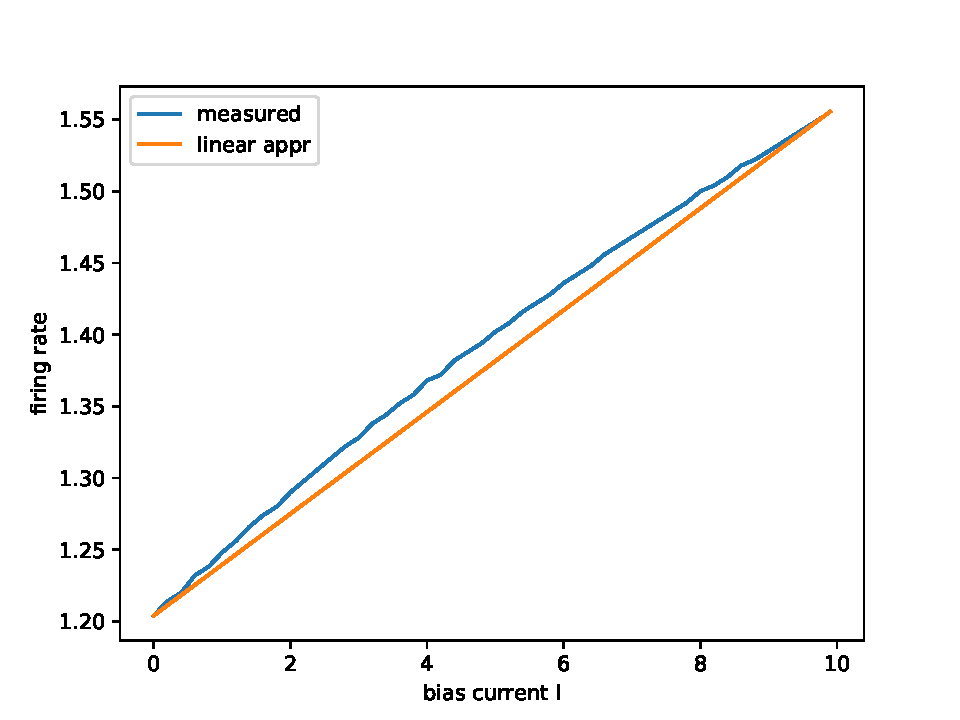
\includegraphics[scale=0.9]{detmocount.pdf} 
	\caption{Verhalten der Feuerrate in Abh"angigkeit vom Bias zwischen 0 und 10 $\mu A/cm^2$}
	\label{count}
\end{figure}
Diese Charakteristik muss nun in allen Rechnungen ber"ucksichtigt werden, die von der Feuerrate abh"angen.
\begin{figure}[H]
	\centering
	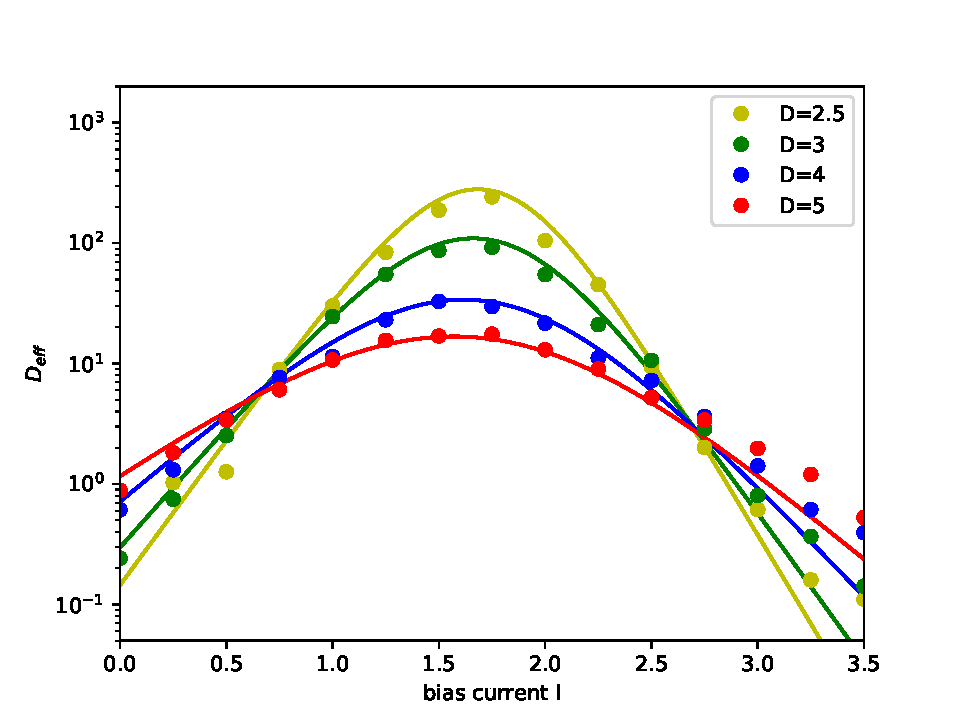
\includegraphics[scale=0.9]{./Bachelorarbeit/bachelorarbeit/dcompdf29m.pdf}
	\caption{Vergleich $D_{eff}$ mit Zwei-Zustands-Modell mit fester Feuerrate}
	\label{dcomp}
\end{figure}
\begin{figure}[H]
	\centering
	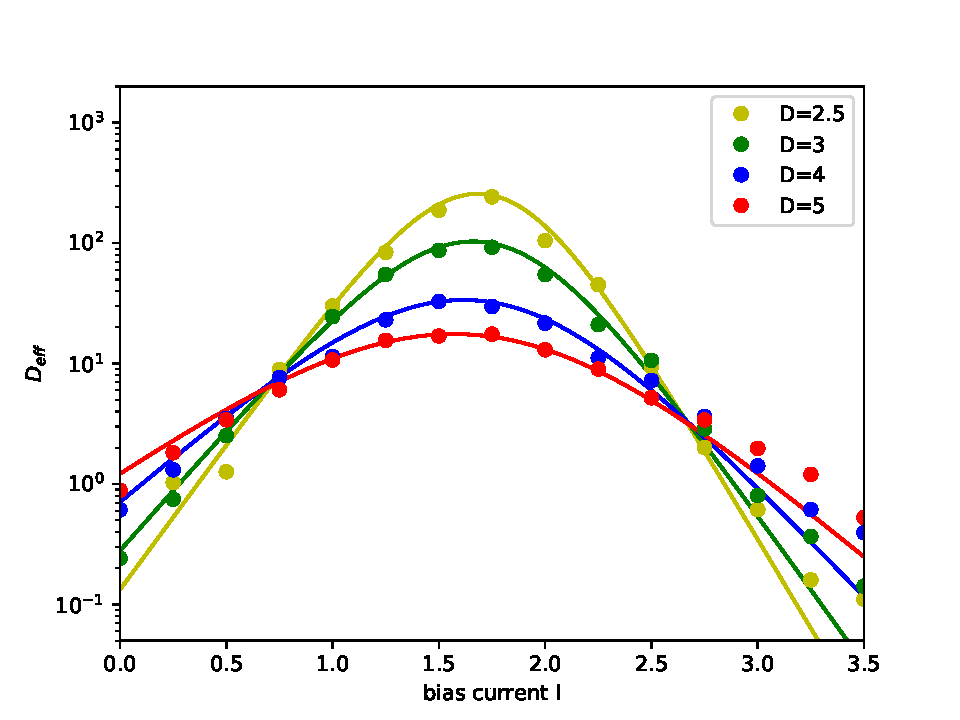
\includegraphics[scale=0.9]{./Bachelorarbeit/bachelorarbeit/dcompdf29mvarv.pdf}
	\caption{Vergleich $D_{eff}$ mit Zwei-Zustands-Modell mit variabler Feuerrate}
	\label{dcompvarv}
\end{figure}
Da sich der Diffusionskoeffizient im betrachteten Bereich um mehrere Gr"o"senordnungen ver"andert, ruft dies hier allerdings nur einen kaum sichtbaren Unterschied hervor.
\section{Verhalten der mittleren Feuerrate}
Wenn das Neuron einem schwachen Signal unterliegt, ist das Signal-zu-Rausch-Verh"altnis proportional zur quadrierten Ableitung der mittleren Feuerrate:
\begin{align*}
SNR \propto \frac{|dr/dI|^2}{D_{eff}}
\end{align*}
Um die Ableitung der mittleren Feuerrate zu berechnen, w"are es hilfreich, einen analytischen Ausdruck f"ur diese zu finden.\\
In der Zwei-Zustands-Theorie l"asst sich die mittlere Feuerrate aus der Feuerrate im burstenden Zustand (die im vorherigen Abschnitt betrachtet wurde) sowie den "Ubergangsraten zwischen den beiden Zust"anden (burstend und ruhend) berechnen:
\begin{align*}
\left<v\right>=v_+\frac{r_-}{r_++r_-}
\end{align*}
wobei
\begin{align*}
r_{\pm}&=r_{0,\pm}\text{e}^{-\frac{\Delta U_{\pm}}{Q}}\\
v_+=a_v*I+b_v
\end{align*}
Die Ableitung kann nun bestimmt werden:
\begin{align*}
\frac{dr}{dI}&=v_+\left(\frac{r_-'}{r_++r_-}-\frac{r_-(r_+'+r_-')}{(r_++r_-)^2}\right)+v_+'\frac{r_-}{r_++r_-}\\
&=v_+\left(\frac{r_+r_-'-r_-r_+'}{(r_++r_-)^2}\right)+a_v\frac{r_-}{r_++r_-}\\
&=v_+\left(\frac{r_+r_-(a_+-a_-)}{Q(r_++r_-)^2}\right)+a_v\frac{r_-}{r_++r_-}
\end{align*}

Aus mehreren Fits (zun"achst mit den Messdaten und dann noch einmal mit den gewonnenen Fitparametern) bekommt man schlie"slich Werte f"ur die Vorfaktoren und Parameter f"ur die linear angen"aherten Potentialbarrieren:
\begin{align*}
r_{0,\pm}&=const\\
\Delta U_\pm&=a_\pm\cdot I+b_\pm
\end{align*}
Vergleicht man dieses Modell mit den tats"achlichen Feuerraten, ist ab einem Strom von $I\approx 2$ eine starke Diskrepanz zwischen Modell und Simulation erkennbar:
\begin{figure}[H]
	\centering
	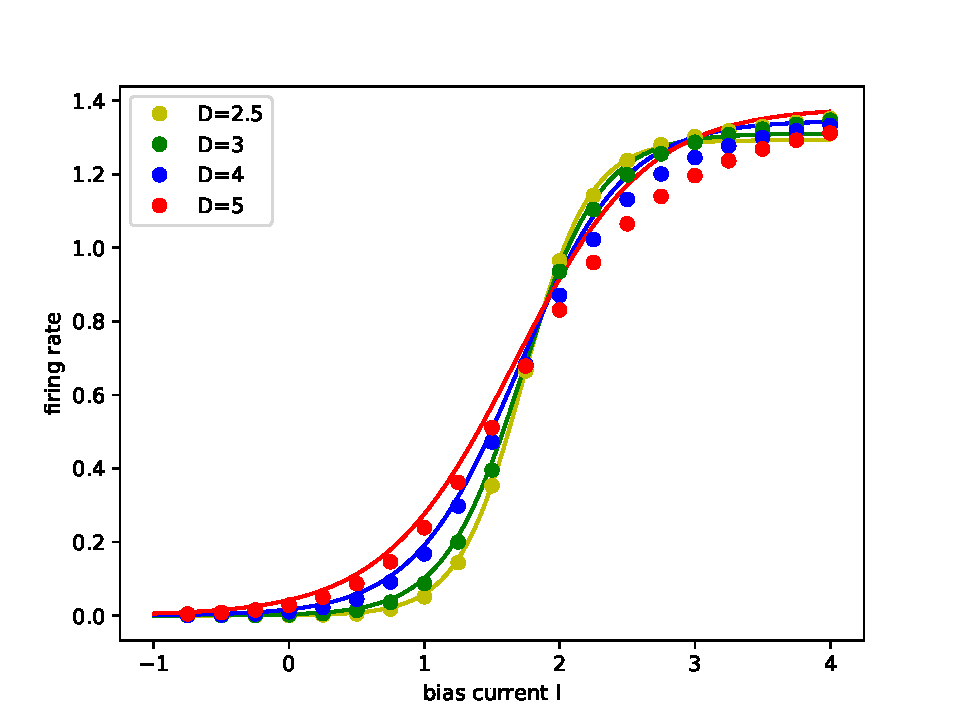
\includegraphics[scale=0.9]{gcompdf29mvarv.pdf}
	\caption{Vergleich der mittleren Feuerrate mit dem Zwei-Zustands-Modell}
	\label{gcompvarv}
\end{figure}
Wenn man den Simulationen hinreichend vertraut, liegt es nahe, lediglich die Simulationsdaten zu fitten, da das Zwei-Zustands-Modell nicht ideal zu sein scheint. Dabei muss allerdings das mathematische Modell etwas kondensiert werden, da:
\begin{align*}
\left<v\right>&=v_+\frac{r_-}{r_++r_-}=\frac{v_+}{1+r_+/r_-}\\
&=\frac{v_+}{1+r_{0,+}/r_{0,-}\exp(-\frac{\Delta U_+-\Delta U_-}{Q})}
\end{align*}
Eine Verwendung des kompletten Modells f"uhrt also zu Overfitting, denn es bleiben nur die relativen Parameter $r_0=r_{0,+}/r_{0,-}$, $a=a_+-a_-$ und $b=b_+-b_-$. Da die Parameter $r_0$ und $b$ nicht voneinander unabh"angig sind, muss einer von ihnen ebenfalls entfernt werden.\\
Mit diesem vereinfachten Modell k"onnen die Messwerte gut gefittet werden:
\begin{figure}[H]
	\centering
	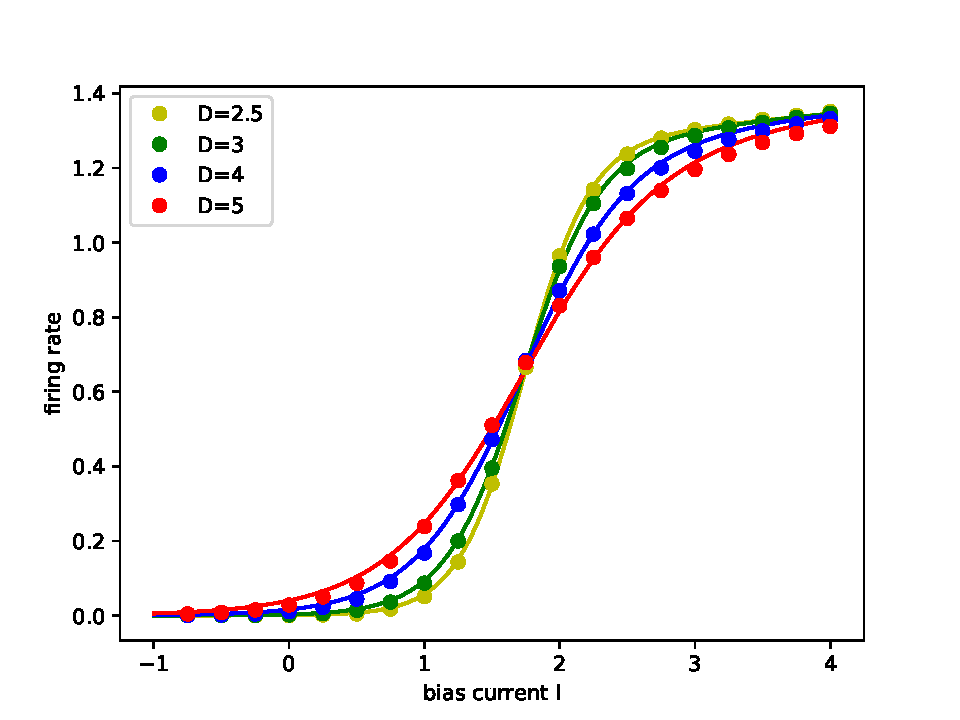
\includegraphics[scale=0.9]{gfit29m.pdf}
	\caption{Fit der mittleren Feuerrate}
	\label{gfit}
\end{figure}
Aus
\begin{align*}
r=\frac{v_+}{1+r_0\exp(-\frac{a\cdot I}{D})}
\end{align*}
erh"alt man f"ur die erste Ableitung:
\begin{align*}
r'=\frac{-v_+\cdot r_0\cdot a \exp(-\frac{a\cdot I}{D})}{D(1+r_0\exp(-\frac{a\cdot I}{D}))^2}+\frac{a_v}{1+r_0\exp(-\frac{a\cdot I}{D})}
\end{align*}



\section{SNR}
\begin{figure}[H]
	\centering
	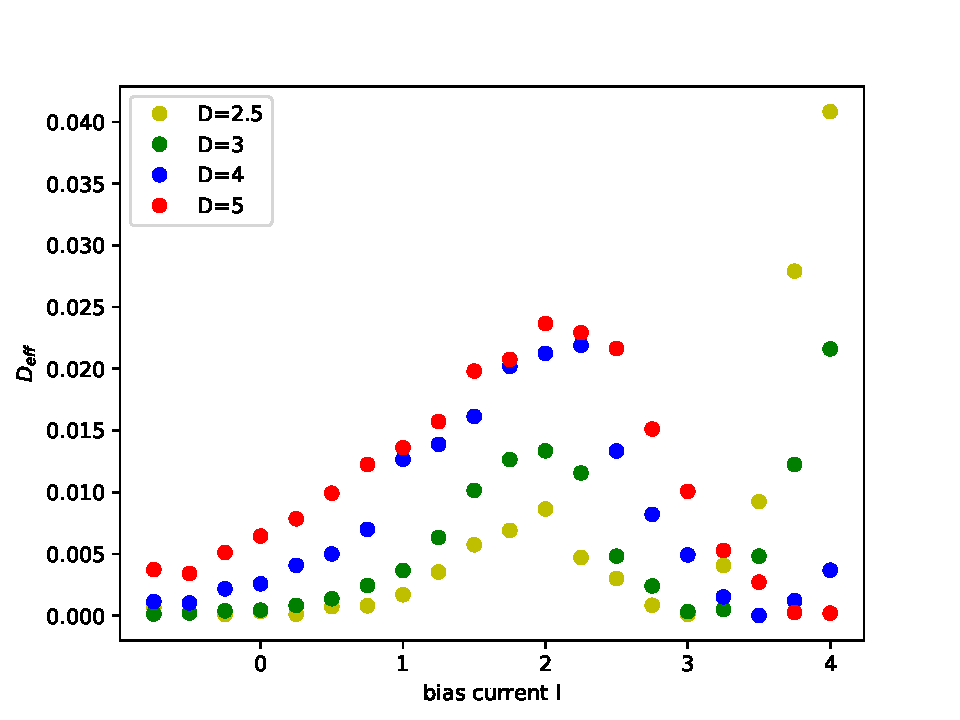
\includegraphics[scale=0.9]{snrcompdf29m.pdf}
	\caption{gen"aherte Ableitung und simuliertes $D_{eff}$}
	\label{snrcomp}
\end{figure}
\begin{figure}[H]
	\centering
	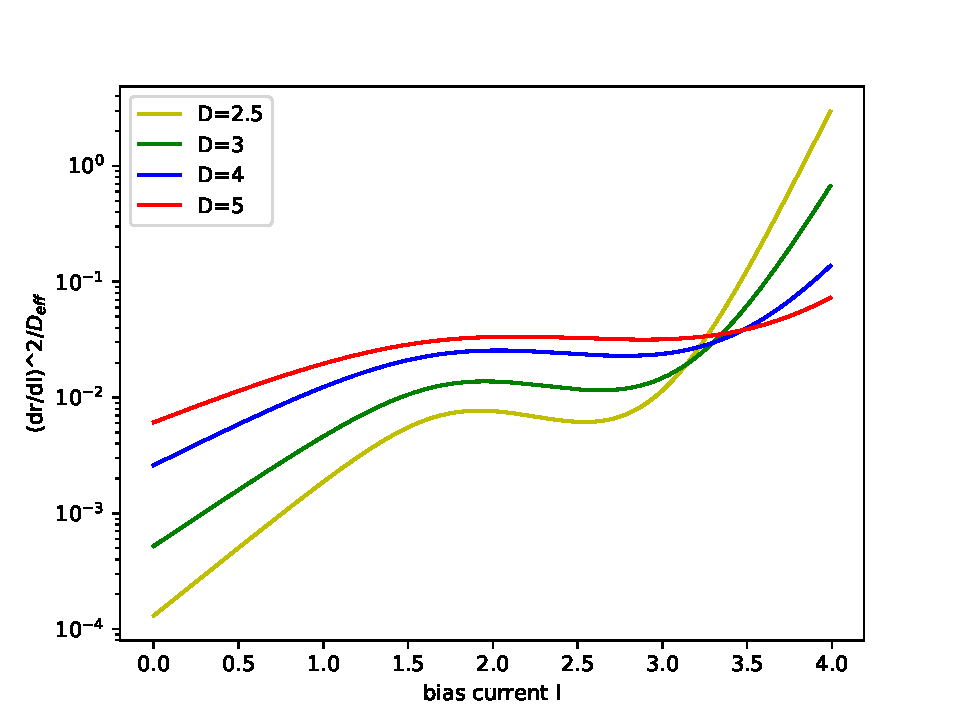
\includegraphics[scale=0.9]{dcompdf29mfull.pdf}
	\caption{Zwei-Zustands-Modell}
	\label{dcompfull}
\end{figure}
\begin{figure}[H]
	\centering
	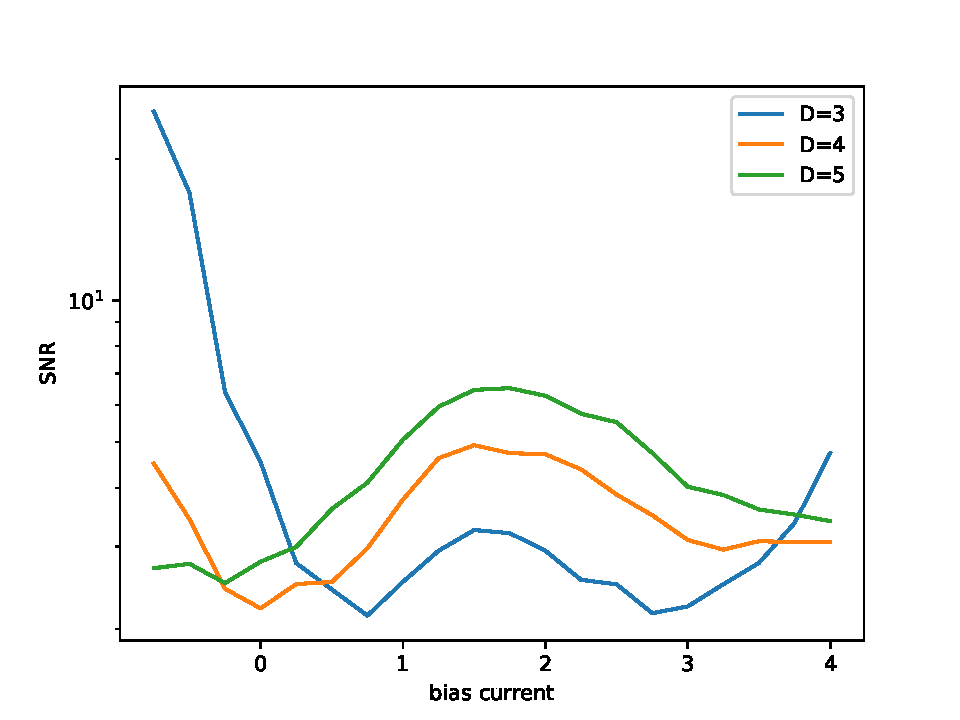
\includegraphics[scale=0.9]{snr345log.pdf}
	\caption{$(dr/dI)^2/D_{eff}$ Simulation}
	\label{snrsim}
\end{figure}
\begin{figure}[H]
	\centering
	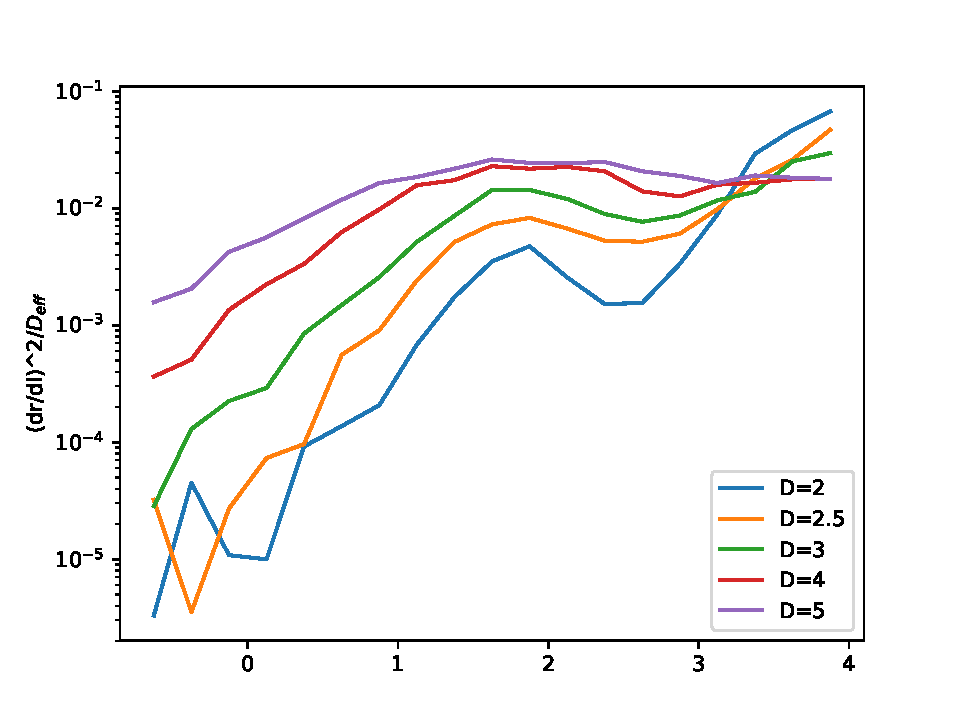
\includegraphics[scale=0.9]{snrapp29m5.pdf}
	\caption{$(dr/dI)^2/D_{eff}$ Absch"atzung: gemessene Ableitung und $D_{eff}$}
	\label{snrapp}
\end{figure}
\end{document}